% Este documento utiliza latex classes disponibilizadas
% no seguinte endereço: http://www.inf.ufrgs.br/utug

\documentclass[tc]{iiufrgs}

\usepackage[brazilian]{babel}
\usepackage{graphicx}
\usepackage[T1]{fontenc}
\usepackage{times}
\usepackage{setspace}
\usepackage{listings}
\usepackage{color}
\usepackage{tabularx}
\usepackage[utf8]{inputenc}

\title{Rivers - Stream Processing API for Golang}

\author{Borges}{Diego}

\advisor[Prof.~Dr.]{Pimenta}{Marcelo}

\date{dezembro}{2015}

\course{Curso de Ciência da Computação}

\location{Porto Alegre}{RS}

\renewcommand{\nominata}{
UNIVERSIDADE FEDERAL DO RIO GRANDE DO SUL
\par Reitor: Prof.~Dr.~Carlos Alexandre Netto
\par Vice-Reitor: Prof.~Dr.~Rui Vicente Oppermann
\par Pró-Reitor de Graduação: Prof.~Dr.~Sérgio Roberto Kieling
\par Diretor do Instituto de Informática: Prof.~Dr.~ Luís da Cunha Lamb
\par Coordenador do Curso de Ciência da Computação: Prof.~Dr.~Raul Fernando Weber
\par Bibliotecária-Chefe do Instituto de Informática: Beatriz Regina Bastos Haro
}

\keyword{API}
\keyword{rivers}
\keyword{golang}
\keyword{stream}
\keyword{pipeline}
\keyword{concurrency}

%
% -----------------------------------------------------------------------------
%

\begin{document}

\maketitle

\clearpage
\begin{flushright}
\mbox{}\vfill
{\sffamily\itshape
``Do not communicate by sharing memory; instead, share memory by communicating''\\}
--- \textsc{Rob Pike}
\end{flushright}

% agradecimentos
\chapter*{Agradecimentos}
\label{cha:thanks}
TODO ...
TODO ...
TODO ...

%
% -----------------------------------------------------------------------------
%

\tableofcontents

% lista de abreviaturas e siglas (o parametro deve ser a abreviatura mais longa):
\begin{listofabbrv}{UFRGS}
        \item[API] Application Programming Interface
        \item[TDD] Test-Driven Development
\end{listofabbrv}

\listoffigures

\listoftables

\begin{abstract}
TODO translation...
During the past few years hardware power has evolved drastically and today's systems can leverage multi-core CPUs in order to perform concurrent tasks more effectively.
Golang takes advantage of this hardware power by implementing a simple message passing concurrency model though extremely powerful using as building blocks channels and what is known as goroutines.
Rivers is a framework for data stream processing built on top of Golang concurrency primitives along with well known patterns such as the Producer-Consumer and the Golang pipeline patterns.
The main goal of this work is to provide a fluent API for building complex data stream pipelines in Golang applying concepts from functional programming.
\end{abstract}

\begin{englishabstract}{Rivers - Stream Processing API for Golang}{API, rivers, golang, stream, pipeline, concurrency}
During the past few years hardware power has evolved drastically and today's systems can leverage multi-core CPUs in order to perform concurrent tasks more effectively.
Golang takes advantage of this hardware power by implementing a simple message passing concurrency model though extremely powerful using as building blocks channels and what is known as goroutines.
Rivers is a framework for data stream processing built on top of Golang concurrency primitives along with well known patterns such as the Producer-Consumer and the Golang pipeline patterns.
The main goal of this work is to provide a fluent API for building complex data stream pipelines in Golang applying concepts from functional programming.
\end{englishabstract}

\onehalfspacing

\chapter{Introdução}
\label{cha:introduction}

\section{Motivação}
\label{sec:motivation}

Nos últimos anos a necessidade de se processar grandes volumes de dados de maneira eficiente e flexível tem aumentado drasticamente. Isso se deve ao fato de que sistemas computacionais estão cada vez mais complexos e frequentemente envolvem a colaboração entre diversos outros sistemas que atuam como fonte ou consumidores de dados. O fato de que as pessoas estão cada vez mais conectadas aos seus dispositivos móveis coletando e produzindo dados a todo momento é um dos indícios dessa crescente complexidade que tende a continuar à medida que novas tecnologias são introduzidas como por exemplo Iternet of Things \cite{blog:iot:council}, aumentando ainda mais a quantidade de dados produzidos e com isso a necessidade de se processar e comunicar estes dados entre os diferentes sistemas que compõem o que conhecemos como Internet.

Dados são gerados assincronamente por diversas fontes como por exemplo aplicativos móveis, sensores, sistemas web e fluem de um sistema à outro através de mecanismos de comunicação tais como APIs e Push Notifications \cite{docs:apple:push_notification} passando por transformações, filtros e agregações para se adequar ao contexto e as necessidades de cada sistema. Todo este processamento quando aplicado a grandes quantidades de dados em um contexto de sistemas distribuídos torna-se surpreendentemente desafiador. Várias soluções foram propostas nos últimos anos para abordar o processamento assíncrono de grandes volume de dados dentre elas o processamento de streams, solução explorada por este trabalho no contexto da linguagem de programação Go da google.

A decisão pelo uso da linguagem de programação Go se deve à alguns fatores. Go introduz um modelo de concorrência poderoso e simples baseado em troca de mensagens através da colaboração entre channels \ref{subsec:channels} e goroutines \ref{subsec:goroutines} permitindo um único programa executar centenas de milhares de fluxos concorrentes de execução com o mínimo de overhead, o que a torna uma linguagem extremamente atraente no contexto de processamento de streams. Go tem ganhado notável adoção na comunidade de desenvolvedores tanto pela simplicidade da linguagem que permite com que soluções elegantes sejam empregadas à problemas complexos como no desenvolvimento de web servers, aplicações que fazem intenso uso de mecanismos de comunicação de rede como TCP e UDP, parsers e etc. No entanto, a linguagem não provê abstrações nativas para o processamento de streams tornando o trabalhado de um desenvolvedor não necessariamente trivial.

\section{Objetivos}
\label{sec:objectives}

Este trabalho tem como principal objetivo a implementação de uma API  simples e flexível para processamento de streams através da abstração de pipelines para a linguagem de programação Go da google. A solução proposta tem como base teórica conceitos do modelo Produtor-Consumidor \cite{paper:david_kocher:producer_consumer} juntamente com conceitos de programação funcional tais como Collection Pipeline definido em \cite{article:martin_fowler:collection_pipeline}. Em sua fundação prática, a solução explora o modelo de concorrência da linguagem Go afim de usufruir ao máximo dos recursos de hardware visando atingir níveis extremos de concorrência e paralelismo.

Visando o reuso de código, a API proposta disponibiliza um conjunto mínimo de abstrações para cada um dos conceitos envolvidos na criação de um pipeline e seus estágios de processamento de stream que servirão como base para a implementação de componentes mais complexos e especializados, tais como mecanismos básicos para a produção de dados de diversas fontes como por exemplo arquivos, sockets e listas e também componentes especializados em operações de transformações de dados como por exemplo Map, Reduce, Filter encontradas em outras soluções similares discutidas no capítulo \ref{cha:related_work}. Afim de adequar-se a cenários não inicialmente previstos Rivers disponibiliza mecanismos para que abstrações nativas da API possam ser estendidas com novas implementações permitindo a criação de pipelines para o processamento de qualquer tipo de dados independente de sua origem.

Finalmente a API proposta seguindo conceitos de programação funcional deve permitir que estágios do pipeline possam ser combinados de maneira simples tal que dados produzidos por um estágio possam ser consumidos por um próximo estágio de maneira assíncrona e concorrente, sendo possível porém opcional a paralelização de estágios específicos afim de aumentar a eficiência de processamento de dados de um estágio em particular.

\begin{flushright}
\mbox{}\vfill
{\sffamily\itshape
``Any fool can write code that a computer can understand. Good programmers write code that humans can understand.''\\}
--- \textsc{Martin Fowler, 2008}
\end{flushright}

\section{Estrutura do Texto}
\label{sec:text_structure}

Este trabalho está organizado em sete capítulos os quais abordam temas relevantes para o entendimento das decisões tomadas no processo de desenvolvimento da solução e suas motivações assim como definição de conceitos básicos utilizados como fundação do trabalho. A seguir cada capítulo é apresentado de maneira mais detalhada.

\begin{description}
    \item [Capítulo~\ref{cha:introduction}] Apresenta o contexto em que o trabalho foi desenvolvido as motivações que justificam a solução proposta assim como seus objetivos.
    \item [Capítulo~\ref{cha:foundation}] Descreve os termos e conceitos básicos utilizados como fundação do trabalho dando suporte teórico e prático para a solução proposta.
    \item [Capítulo~\ref{cha:related_work}] Discute alguns trabalhos relacionados que serviram de base e inspiração para muitas das decisões técnicas tomadas ao longo do processo de desenvolvimento deste trabalho.
    \item [Capítulo~\ref{cha:rivers}] Apresenta a solução proposta em detalhes assim como a arquitetura desenvolvida e seus componentes internos
    \item [Capítulo~\ref{cha:rivers_implementation}] Descreve o processo de desenvolvimento empregado assim como as práticas utilizadas para a validação gradual de requisitos assim como a integração contínua e constante da implementação empregada.
    \item [Capítulo~\ref{cha:applications}] Apresenta alguns casos de uso detectados ao longo do desenvolvimento assim como aplicações reais da solução em ambientes de produção juntamente como a visão de desenvolvedores que fizeram para da validação deste trabalho.
    \item [Capítulo~\ref{cha:conclusion}] Por fim, são apresentados as conclusões, resultados e algumas considerações finais com relação a possíveis melhorias e avanços futuros.
\end{description}

\chapter{Estado da Arte}
\label{cha:state_of_art}

TODO: brief overview of the Golang concurrency model and its challenges ...


\chapter{Trabalhos Relacionados}
\label{cha:related_work}

A seguir serão descritos brevemente alguns projetos que inspiraram a criação de Rivers não necessariamente relacionados à linguagem Go mas que aplicam conceitos similares para processamento de dados frequentemente no formato de streams.

\section{Apache Spark}
\label{sec:apache_spark}

Achache Spark \cite{docs:apache:spark} é uma solução para computação de tempo real, tolerante a falhas e com suporte a clustering \cite{article:kris:clustering}, com APIs em diferentes linguagens de programação como por exemplo scala, java e python. Spark tornou-se muito popular em áreas de \emph{Machine Learning} \cite{course:coursera:ml} e \emph{Analytics} \cite{article:techtarget:analytics} devido ao seu grande poder computacional que permite que grandes volumes de dados possam ser processados e distribuídos em diferentes máquinas de um cluster sendo uma solução muito atrativa também para sistemas de processamento de eventos \cite{docs:apache:streaming}.

\begin{figure}[H]
  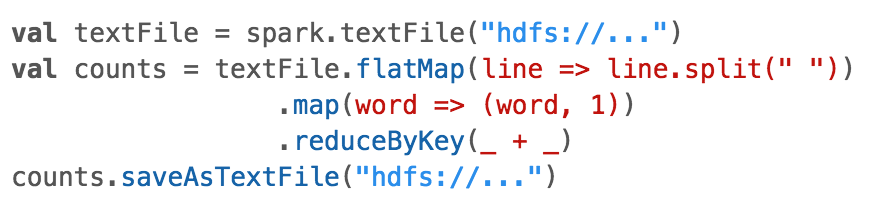
\includegraphics[width=0.7\textwidth]{spark}
  \centering
  \caption{Exemplo de uso da API scala de Spark.}
  \label{code:apache:spark}
\end{figure}

A API de Rivers é fortemente inspirada na fluência da API Spark, aplicando \emph{Method Chaining} \cite{article:sitepoint:method_chaining} sempre que possível aumentando a legibilidade do código resultante. Ambas APIs aplicam ao máximo os conceitos de programação funcional disponibilizando operações de filtros, mapeadores e agregadores de dados provendo um considerável nível de composição entre operações permitindo a criação de pipelines complexos de processamento de streams fortemente suscetíveis ao reuso. Suporte à clustering em Rivers é proposto como parte de trabalhos futuros.

\section{Java 8 Streams}
\label{sec:java8_streams}

A versão 8 da linguagem de programação Java introduz a abstração de Streams \cite{docs:java8:streams} como parte de suas bibliotecas padrão e assim como outras linguagens e plataformas como Spark, disponibiliza uma API fluente baseada em conceitos de programação funcional, permitindo a criação de pipelines para processamento de streams com suporte a paralelização. Assim como Spark, a API de streams de Java8 contribuíram para o design da API de Rivers afim de prover uma API similar para a linguagem Go que não fosse somente simples porém familiar à desenvolvedores com conhecimentos de programação funcional e extensível permitindo que a solução fosse aplicada à novos casos de uso introduzindo implementações diferentes dos componentes básicos do framework \ref{sec:rivers:building_blocks}.

\begin{figure}[H]
  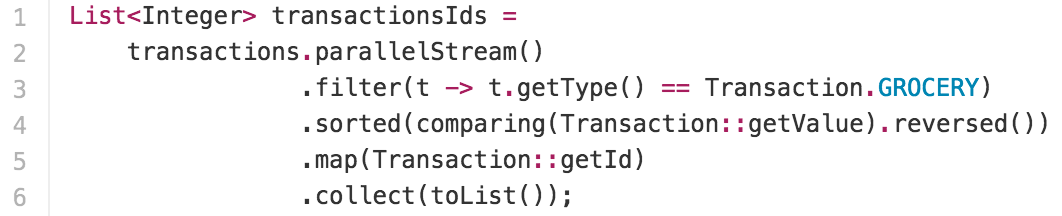
\includegraphics[width=0.9\textwidth]{java8_streams}
  \centering
  \caption{Exemplo de uso da API de streams em Java8.}
  \label{code:java8:streams}
\end{figure}

\section{ReactiveX - Reactive eXtensions}
\label{sec:reactive_extensions}

\emph{Reactive eXtensions} \cite{docs:reactivex:streams} é um movimento que tomou tração nos últimos anos liderado por empresas como \cite{netflix} e \cite{microsoft} dentre outras que procura tornar \emph{mainstream} conceitos de programação reativa \cite{article:reactive_programming} empregando vários conceitos de programação funcional e conhecidos padrões de design como \emph{Observer Pattern} \cite{article:pattern:observer} e \emph{Observable Pattern} \cite{article:pattern:observable} na criação de APIs assíncronas para tratamento de fluxo de dados. Estes conceitos quando combinados permitem com que APIs poderosas sejam implementadas abstraindo muito dos desafios envolvidos na programação assíncrona como por exemplo sincronização de threads, estruturas de dados concorrentes e operações de IO não bloqueantes. Existem várias implementações da especificação dentre elas estão a API Java \cite{docs:javarx} e Javascript \cite{docs:javascriptrx}.

Apesar de Rivers não seguir necessariamente a especificação de Reactive eXtensions, muitas decisões de design em Rivers foram baseados em conceitos similares aplicados à RX, como por exemplo realização de \emph{back-pressure} \cite{article:tim:streams} do pipeline através da utilização de Go \emph{buffered channels} \cite{docs:go:buffered_channels}. Reactive eXtensions e outros casos de uso explorados neste capítulo mostram que processamento de streams é uma solução interessante para muitos problemas relacionados a diversas áreas tecnológicas como por exemplo Big Data, Analytics, Event Processing e muitas linguagens de programação adotaram estes conceitos de provendo APIs nativas que permitem com que pipeline de processamento de streams sejam criados de maneira simples abstraindo muito dos desafios envolvidos com relação a concorrência e paralelização de um pipeline por exemplo, motivando a criação de Rivers.

\begin{flushright}
\mbox{}\vfill
{\sffamily\itshape
``ReactiveX is more than an API, it's an idea and a breakthrough in programming. It has inspired several other APIs, frameworks, and even programming languages.''\\}
--- \textsc{ReactiveX.io}
\end{flushright}


\chapter{Rivers: Arquitetura}
\label{cha:rivers_architecture}

TODO - Brief Overview on the main architectural aspects:

\section{Building Blocks}
\label{sec:building_blocks}

TODO

Composition + Rivers Flow: From -> Apply -> Then

\section{Pipeline Pattern}
\label{sec:the_pipeline_pattern}

TODO ...

Achieving concurrency with pipeline pattern

\section{The Cancellation Problem}
\label{sec:the_cancellation_problem}

TODO ...

\section{Producers}
\label{sec:producers}

TODO ...

\section{Consumers}
\label{sec:consumers}

TODO ...

\section{Transformers}
\label{sec:transformers}

TODO ...

\section{Combiners}
\label{sec:combiners}

TODO ...

\section{Dispatchers}
\label{sec:dispatchers}

TODO ...

\section{Going Parallel}
\label{sec:going_parallel}

TODO ...

Concurrency is not parallelism

Talk about how Rivers achieve parallelism within a pipeline stage

Refer to http://blog.golang.org/concurrency-is-not-parallelism, use the gopher diagrams to make the idea clear

Benchmarks?

\section{The Error Recovering Mechanism}
\label{sec:recovering_mechanism}

TODO

Error scenarios + deadline timeouts

Golang Panic + Recover

Overriding the recovering function

The Debug Mode + Stacktrace

\section{Extending Rivers}
\label{sec:extending_rivers}

TODO

\subsection{Writing Custom Producers}
\label{sec:custom_producers}

TODO

\subsection{Writing Custom Consumers}
\label{sec:custom_consumers}

TODO

\subsection{Writing Custom Combiners}
\label{sec:custom_combiners}

TODO

\subsection{Writing Custom Dispatchers}
\label{sec:custom_dispatchers}

TODO


\chapter{Conclusão}
\label{cha:conclusion}

Rivers propões uma API simples, extensível e intuitiva para processamento de streams de dados para a linguagem Go, utilizando de construções e conceitos de programação funcional familiares a maioria dos desenvolvedores abstraindo as complexidades e detalhes de implementação relacionados ao processamento concorrente e paralelo dos dados, de maneira que o desenvolvedor passa se concentrar apenas na lógica de negócio intrínseca ao pipeline.

O modelo de concorrência da linguagem Go provou-se não somente muito conveniente mas também extremamente eficiente e foi crucial para o sucesso da implementação da solução uma vez que muito da complexidade dos mecanismos de detecção de falhas, de comunicação entre os componentes do sistema via channels e gerência de recursos alocados durante a execução de grandes quantidades de fluxos de processamento concorrentes não afetaram de maneira considerável a complexidade final da solução.

Por se tratar de um experimento e guiado inicialmente pelas necessidades e casos de uso da emprese Bearch Inc, a API sofreu várias alterações ao longo do desenvolvimento afim de adaptá-la a novos casos de uso, porém visando simplicidade algumas operações encontradas em APIs similares em outras plataformas não foram implementadas como por exemplo determinados tipos de operações de filtros que no entanto podem ser implementadas através da composição de outras operações disponíveis na API.

\section{Análise dos Resultados}
\label{sec:results}

Ao longo do desenvolvimento muitas informações foram coletadas desde benchmarks até feedbacks de desenvolvedores utilizando o framework em outros projetos da empresa afim de avaliar a solução em termos de performance, simplicidade e flexibilidade. Os resultados dos benchmarks foram muito satisfatórios e mostraram um ganho considerável em performance ao se paralelizar estágios do pipeline além da execução concorrente de cada estágio.

O design funcional da API agradou desenvolvedores pela simplicidade da solução e o fato de se poder estender a API com novos componentes implementando as interfaces definidas pelo framework possibilitou o uso de Rivers em contextos bem variados. Algumas das decisões técnicas quanto ao design da API foram guiados por feedbacks de usuários que alongo de várias conversas e experimentos ajudaram a moldar a API final desde a nomenclatura das operações até mesmo com relação a melhor solução para se paralelizar pipelines sem expor qualquer tipo de complexidade ao usuário do framework. Um ponto negativo levantado por desenvolvedores é que devido ao fato da sintaxe da linguagem Go em alguns aspectos é um pouco extensa comparado com outras soluções em outras linguagens como scala e python, é necessário escrever um pouco mais de código, porém isso pode ser contornado fornecendo implementações específicas de operações recorrentes que possam ser reusadas evitando a necessidade de se implementar a mesma funcionalidade em diferentes contextos.

\section{Trabalhos Futuros}
\label{sec:future_work}

Ao longo do desenvolvimento da solução, alguns casos de uso interessantes foram detectados, propostos e discutidos como por exemplo a possibilidade de se implementar pipelines distribuídos, permitindo a execução de diferentes estágios do pipeline em um cluster de máquinas seguindo um modelo similar ao modelo MapReduce proposto por Google \cite{paper:google:map_reduce}. Apesar de ser um caso de uso muito interessante, a complexidade de implementação não justificou sua necessidade momentânea e portanto não foi considerado prioridade no desenvolvimento. Porém essa possibilidade não foi completamente descartada e fica proposta como trabalho futuro uma vez que existem necessidades reais que justificam o investimento em tal solução, especialmente nos domínios de Big Data aonde o volume de dados a serem processados é incrivelmente grande e a possibilidade de se distribuir e processar conjuntos menores destes dados em diferentes máquinas agregando seus resultados ao final é muito atraente.

%
% -----------------------------------------------------------------------------
%

\bibliographystyle{abnt}
\bibliography{chapters/references}

\end{document}
